\section{Què és?}

	Anomenem software privatiu a tot aquell programa publicat sota llicències
	que reserven un o tots els drets d'ús, còpia, modificació i distribució
	al fabricant qui, pagant, concedeix un ús del programa executable al titular
	de la llicència.

	Per tant, el software \emph{privatiu} o \emph{propietari} obstrueix la llibertat
	de l'usuari final, que quan ha adquirit el programa, té uns drets limitats i fortes
	obligacions, que solen incloure la impossibilitat d'adquirir i modificar el codi font del producte
	que ell mateix ha comprat, tant com la prohibició total o parcial de la redistribució del programa.
	\cite{gnucategories}

	Per a entendre millor el software propietari, posem un exemple pràctic (i desgraciadament, verídic).
	La nova consola de Sony, la \emph{PlayStation 4}, posseeix un \emph{sistema operatiu} \footnote{Conjunt
	de programes i funcions que fan funcionar un ordinador.} privatiu que es basa alhora en un sistema operatiu
	anomenat \emph{FreeBSD}, de llicència no-privativa \cite{freebsdlicense}. Aquest sistema operatiu, FreeBSD, té una
	quantitat d'usuaris i de desenvolupadors molt baixa, el que dificulta el desenvolupament de \emph{drivers}, que
	permetran el millor funcionament de diferents components d'un ordinador amb el sistema operatiu. La llicència que FreeBSD utilitza, permet
	la revocació de la llicència per la substitució d'una altra, i això és el que ha aprofitat Sony: realitzarà millores
	sobre el sistema operatiu, i ningú dins la comunitat d'usuaris de FreeBSD se'n podrà beneficiar, ja que ara és Sony qui
	fa el que vol amb el producte lliure que ha adquirit i modificat. D'aquesta forma, l'evolució del OS \footnote{Sistema operatiu}
	FreeBSD és molt més lenta que, per exemple, l'evolució dels sistemes operatius \emph{GNU/Linux}, que utilitzen
	una llicència diferent.

\section{Qui el fa?}

	El principal desenvolupador de software privatiu a nivell mundial és \emph{Microsoft}, encara que hi
	ha moltes més empreses que també en creen i distribueixen, com \emph{Apple, Oracle, Adobe, VMware,
	SAP, Symantec...} \cite{privatiuempreses}

\section{Ús actual}

	Avui en dia molta part del software utilitzat per la majoria de població, és privatiu.

	Aquesta gran extensió del seu ús és degut a l'inversió milionària al màrketing, i a
	pactes amb productors de sistemes operatius i proveïdors d'Internet, que acorden la
	prèvia instal·lació de software privatiu als ordinadors. La falta d'informació per
	part de la major part d'usuaris fa que aquest fet sigui de poca importància.

	\begin{figure}[ht!]
	\centering
	\includegraphics[width=100mm]{data/web_servers_share.png}
	\caption{Ús de software privatiu/lliure \cite{whyfoss}}
	\label{websshare}
	\end{figure}

	\begin{figure}[h!]
	\centering
	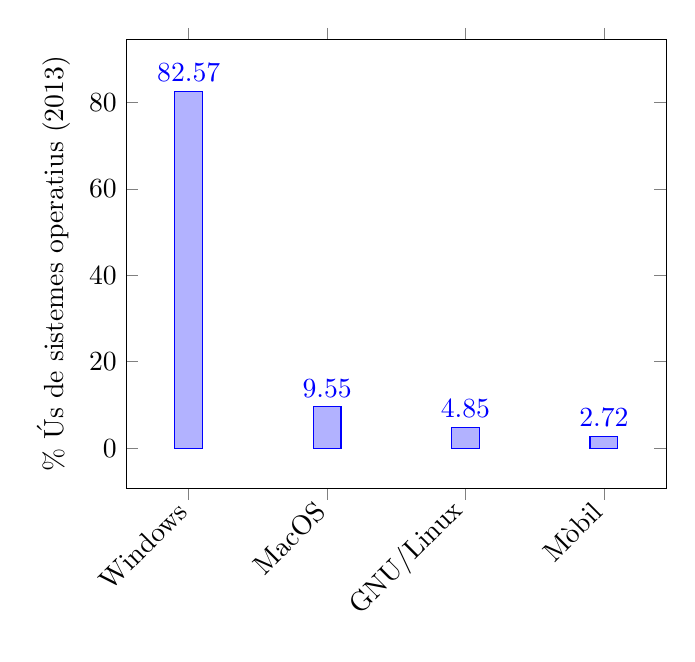
\begin{tikzpicture}
	\begin{axis}[
		ybar,
		enlargelimits=0.15,
		legend style={at={(0.5,-0.2)},
		anchor=north,legend columns=-1},
		ylabel={\% Ús de sistemes operatius (2013)},
		symbolic x coords={Windows,MacOS,GNU/Linux,Mòbil},
		xtick=data,
		nodes near coords,
		nodes near coords align={vertical},
		x tick label style={rotate=45,anchor=east},
	]
	\addplot coordinates {(Windows,82.57) (MacOS,9.55)
	(GNU/Linux,4.85) (Mòbil,2.72)};
	\end{axis}
	\end{tikzpicture}
	\caption{Ús de sistemes operatius per a particulars \cite{osstats}}
	\label{osshare}
	\end{figure}

	\begin{figure}[h!]
	\centering
	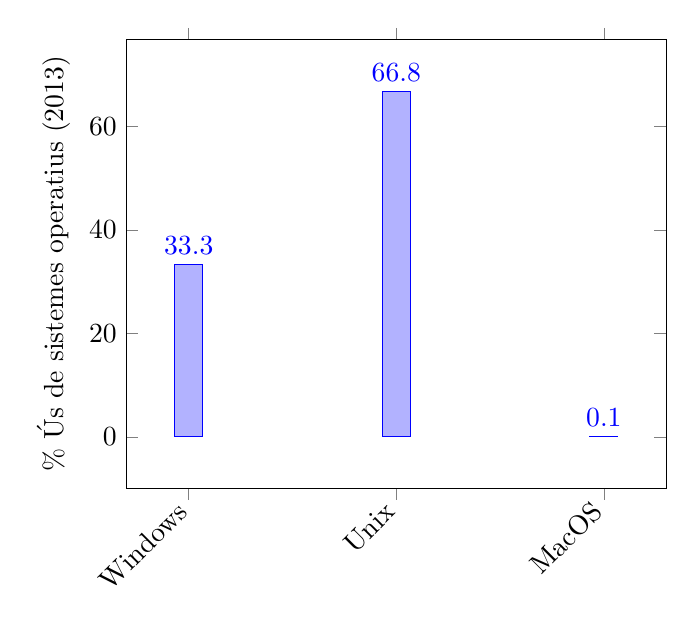
\begin{tikzpicture}
	\begin{axis}[
		ybar,
		enlargelimits=0.15,
		legend style={at={(0.5,-0.2)},
		anchor=north,legend columns=-1},
		ylabel={\% Ús de sistemes operatius (2013)},
		symbolic x coords={Windows,Unix,MacOS},
		xtick=data,
		nodes near coords,
		nodes near coords align={vertical},
		x tick label style={rotate=45,anchor=east},
	]
	\addplot coordinates {(Unix,66.8) (Windows,33.3) (MacOS,0.1)};
	\end{axis}
	\end{tikzpicture}
	\caption{Ús de sistemes operatius per a servidors \cite{ossvstats}}
	\label{ossvshare}
	\end{figure}

	El gràfic \ref{websshare} mostra la distribució (o \emph{market share}) de diferents companyies de software
	en l'àmbit dels servidors web
	\footnote{Ordinadors que funcionen el màxim de temps possible i comparteixen l'accés a una direcció web.
	Per exemple, \emph{Google} té molts servidors que permeten l'accés públic als seus serveis.}.
	\emph{Apache}\cite{apache} ha mantingut sempre la seva posició,
	seguit per \emph{Microsoft} i altres companyies. En aquest cas, el software lliure (de la mà de la
	llicència \emph{Apache 2.0}\cite{apachelicense}) és prevalent de llarg.

	El gràfic \ref{osshare} mostra el market share de \emph{sistemes operatius} que utilitzen els particulars
	(qualsevol persona). \emph{Microsoft Windows} és el guanyador indiscutible, amb \emph{MacOS} molt per darrere
	i els sistemes operatius \emph{GNU/Linux} amb menys del 5\% del share.

	El gràfic \ref{ossvshare} mostra el market share de sistemes operatius que utilitzen els servidors


\section{Avantatges del software propietari}

Ventatges del software privatiu: 

-Propietat i decissió de l'ús del software per part de la empresa: fer un bon software 
requereix una important inversió econòmica que, si fos lliure, no serviria de res ja 
que just quan l'acabéssim, la competència es podria apropiar del mateix.

-Solen tenir millor acabat que el software lliure: en el software lliure, degut a que
 el fa molta gent sol tenir diferències de format i no tenen tan bon acabat (tot i que
 molts softwares lliures tenen molt bon acabat).

-Les aplicacions actuals amb més èxit al mercat són, en majoria, propietaries.

-Més possibilitats en el mercat laboral: en la majoria de les feines d'informàtica la
feina que es durà a terme serà en el softwafare privatiu.
\cite{gentegeek}








